\documentclass[../main.tex]{subfiles}
\graphicspath{
		{"../img/"}
		{"img/"}
}

\begin{document}
Uzupełnienie:\\
Na ostatnim wykładzie wprowadziliśmy wielkość
\[
		\overline{u} (x,r,t) = \frac{1}{4\pi r^2}\int\limits_{|x'|=r}u(x+x',t)d s'
,\]
która spełniała równanie
\begin{equation}
		\label{eq:falowe}
		\overline{u} _{,t t}(x,r,t) = c^2 \frac{\partial ^2}{\partial r^2} \overline{u} (x,r,t) + 2c^2 \frac{1}{r} \frac{\partial }{\partial r} \overline{u} (x,r,t)
\end{equation}
Podczas dowodu doszliśmy (dzięki tożsamości Greena) do zależności:
\begin{equation}
		\label{eq:kwiatek}
		\int\limits_{0}^{r}\left( r' \right) ^2 dr' \int\limits_{\text{kąty}} u_{,t t} = r^2c^2 \int\limits_{\text{kąty}} \frac{\partial u}{\partial r}
\end{equation}
teraz różniczkujemy po $r$
\begin{equation}
		\label{eq:kirchoff}
		r^2 \int\limits_{\text{kąty}} u_{,t t} = 2 r c^2 \int\limits_{\text{kąty}} u_{,r}+ r^2 c^2 \int\limits_{\text{kąty}} u_{,rr}
\end{equation}
\begin{pytanie}
		jak ze wzoru \ref{eq:kirchoff} przejść do wzoru \ref{eq:falowe}?\\
		Zauważmy, że
		\begin{align*}
				\overline{u} (x,r,t) &= \frac{1}{4\pi r^2} \int d\theta'\sin\theta' \int d\varphi u(r_0+r, \theta_0+\theta', \varphi_0+\varphi')r^2 = \\
				&= \frac{1}{4\pi}\int d\theta' \sin\theta' \int d\varphi u(r_0+r, \theta_0+\theta', \varphi_0+\varphi') = \\
				&= \frac{1}{4\pi}\iint\limits_{\text{kąty}} u(r_0+r,\ldots)
		.\end{align*}
\end{pytanie}
Popatrzmy na wzór \ref{eq:kwiatek}. Jeżeli wyciągniemy $\frac{\partial }{\partial r} $ przed całkę, to:
\[
		\int\limits_0^r \left( r' \right) ^2 dr' \int\limits_{\text{kąty}, \partial K(0,1)}u_{,t t} = r^2 c^2 \frac{\partial }{\partial r} \int\limits_{\text{kąty}}u
.\]
\[
		\int\limits_0^r \left( r' \right) ^2 dr' \overline{u} (r',t,x) = r^2 c^2 \frac{\partial }{\partial r} \overline{u} (r,t,x)
.\]
To teraz zróżniczkować po $r$ i już
\[
		r^2 \overline{u} (r,x,t) = \frac{\partial }{\partial r} \left( r^2c^2 \overline{u} _{,r} \right)
.\]
\subsection{Zasada Huygensa}
Jak przełożyć na język matematyki możliwość nadawania morsem? Co to znaczy, że ktoś uderzył w stół? Widzimy, że z punktu widzenia (słyszenia) odbiorcy to jest tak, jakby warunki początkowe zmieniały się w czasie. Jak przełożyć taki problem na język, który poznaliśmy?
My umiemy tak:
\[
		u(x,0) = f(x)\quad u_{,t}(x,0) = g(x)
.\]
\begin{figure}[h]
		\centering
		\includegraphics[width=0.8\textwidth]{nadawanie-morsem}
		\caption{Zauważmy, że normalnie, to oba rysunki dają ten sam efekt}
		\label{fig:nadawanie-morsem}
\end{figure}
Czyli zamiast jednego krasnala z instrukcją (trzymaj naciśnięte 5 sekund), ustawiamy w rzędzie ileś krasnali (ostatni będzie oddalony o dajmy na to $5 \times 3 \times 10^8$ m) i każemy błysnąć ultrakrótko, a te wszystkie błyski złożą się w naszym oku w błysk pięciosekundowy.\\
\begin{pytanie}
		To kiedy w końcu można nadawać morsem?
\end{pytanie}
Kiedy warunek brzegowy zlokalizowany przestrzennie da się zlokalizować czasowo, w tym sensie, że dla nas później go nie ma. Wyobraźmy sobie sytuację, w której uderzenie w stół dźwięczy cały cas w powietrzu, a błysk światła nie zanika (gdzieś obok jest pytanie dlaczego niebo w nocy jest czarne). Czyli przeszłość się ciągnie jak adres e-mailowy założony przez 12-latka. Koszmar, prawda?\\
\begin{tw}
		(Obserwacja - Zasada Huygensa)\\
		Niech $f$ i $g$ - funkcje o nośniku zwartym.
		\begin{align*}
				\supp f &= \left\{ x\in \mathbb{R}^3, f(x) \neq 0 \right\}\\
				\supp g &= \left\{ x\in \mathbb{R}^3, g(x) \neq 0 \right\}
		\end{align*}
		i niech $s = \supp f \cup \supp g$. Wówczas $u(x,t) = 0 \underset{t\in [t_1(x),t_2(x)]}{\forall},$ gdzie
		\begin{align*}
				t_1(x) &= \underset{t}{\inf} \left\{ t>0, s^2(x,ct) \cap s \neq \phi \right\}\\
				t_2(x) &= \underset{r}{\inf} \left\{ t>0, s^2(x,ct) \cap s \neq \phi \right\}
		.\end{align*}
		(Brzeg sfery czterowymiarowej jest trójwymiarowy). \\
\end{tw}
		\textbf{Uwaga:} w.w. warunek działa tylko wtedy, gdy rozwiązanie spełnia zasadę Huygensa.
		\begin{figure}[h]
				\centering
				\includegraphics[width=0.4\textwidth]{kule}
				\caption{zasada Huygensa}
				\label{fig:kule}
		\end{figure}
		\begin{przyklad}
				Popatrzmy na problem 3-D:
				\[
						u(x,t) = \frac{1}{4\pi c^2} \left[ \frac{\partial }{\partial t} \left( \frac{1}{t}\int\limits_{\partial K(x,ct)}f(s)d s \right)  \right] + \frac{1}{4\pi^2c^2 t}\int\limits_{\partial K(x,ct)}g(s)d s
				.\]
				Widzimy, że jeżeli $s^2(x,ct)\land \supp f = \phi$, to całka da nam zero.
		\end{przyklad}
		\begin{przyklad}
				Problem 1-D:
				\[
						u(x,t) = \frac{f(x-ct) + f(x+ct)}{2} + \frac{1}{2c}\int\limits_{x-ct}^{x+ct}g(\xi)d\xi
				.\]
		\end{przyklad}
		Chcemy rozwiązać następujący problem
		\begin{align*}
				u_{,t t} &= c^2 \Delta u,\quad u: \mathbb{R}_+ \times \mathbb{R}^2 \to \mathbb{R}\\
				u(x,y,0) &= f(x,y)\\
				u_{,t}(x,y,0) &= g(x,y)
		.\end{align*}
		Czyli problem dwuwymiarowy. Zauważmy, że fajne rozwiązanie moglibyśmy dostać z Kirchoffa, wkładając do niego warunki początkowe zależne od $z$:
		\[
				u(x,y,t) = \tilde u(x,y,z,t) = \frac{1}{4\pi c^2}\frac{\partial }{\partial t} \left[ \frac{1}{t}\int\limits_{|x'| = ct}f(x+x')d s' \right]
		.\]
		Czyli chodzi o wycałkowanie funkcji
		\[
				\int\limits_{(x')^2 + (y')^2 + (z')^2 = (ct)^2}f(x+x',y+y')d s'
		.\]
		Pamiętamy, że z macierzy Grama mieliśmy
		\[
				d s = \sqrt{1+\left( \frac{\partial z}{\partial x}\right) ^2 + \left(\frac{\partial z}{\partial y}  \right) ^2}
		.\]
		Skoro $(z')^2 = (ct)^2 - (x')^2 - (y')^2$, to
		\[
				\frac{\partial z'}{\partial x'} = \frac{-2x'}{2\sqrt{(ct)^2 - (x')^2 - (y')^2} },\quad \frac{\partial z'}{\partial y'} = \frac{-2y'}{2\sqrt{(ct)^2 - (x')^2 - (y')^2} }
		.\]
		Zatem
		\begin{align*}
				(d s)^2 &= 1 + (z_{,x})^2 + (z_{,y})^2 = \\
				&= \frac{(ct)^2 - (x')^2 - (y')^2 + (x')^2 + (y')^2}{(ct)^2 - (x')^2 - (y')^2} = \frac{(ct)^2}{(ct)^2 - (x')^2 - (y')^2}
		.\end{align*}
		Czyli teraz jak podstawimy to dostaniemy (pamiętamy, że jak mapujemy sferę na płaszczyznę, to bierzemy płat z góry i płat z dołu)
		\begin{align*}
				u(x,y,t) &= \frac{2\cdot 1}{4\pi c^2} \frac{\partial }{\partial t} \left( \frac{1}{t}\int\limits_{(x')^2 + (y')^2 \le (ct)^2} \frac{f(x+x',y+y')dx'dy'(ct)}{\sqrt{(ct)^2 - (x')^2 - (y')^2}} \right) + \\
				&+ \frac{2 \cdot 1}{4\pi c^2} \frac{1}{t}(ct) \int\limits_{(x')^2 + (y')^2 \le (ct)^2} \frac{g(x+x', y+y')dx'dy'}{\sqrt{(ct)^2 - (x')^2 - (y')^2}}
		.\end{align*}
		\begin{pytanie}
				Co z zasadą Huygensa?
		\end{pytanie}
		Zauważmy, że wartość rozwiązania w punkcie $(x,y,t)$ zależy od całki po wnętrzu kuli $(x')^2 + (y')^2 \le (ct)^2$, czyli sygnał nigdy nie zniknie! (oczywiście, kiedy mówimy o falach biegnących).
		\begin{pytanie}
				Czy tą samą metodą możemy przejść z 2-D do 1-D?
		\end{pytanie}
		Powinniśmy założyć, że $f(x,y)$ zależy tylko od $x$ i włożyć to do wzoru 2-D:
		\begin{align*}
				u(x,t) &= \frac{1}{2\pi c^2} \frac{\partial }{\partial t} \int\limits_{(x')^2 + (y')^2 \le (ct)^2} \frac{f(x+x')dx'dy'}{\sqrt{(ct)^2 - (x')^2 - (y')^2}} = \\
				&= \frac{1}{2\pi c^2} \frac{\partial }{\partial t} \int\limits_{-ct}^{ct}dx' f(x+x') \cdot 2 \int\limits_0^{\sqrt{(ct)^2 - (x')^2} } \frac{dy'}{\sqrt{(ct)^2 - (x')^2 - (y')^2}}
		.\end{align*}
		Pamiętamy, że mamy wzorek
		\[
				\int\limits_0^r \frac{dy'}{\sqrt{r'^2 - (y')^2}}  = \left.\arcsin\left( \frac{y'}{r'} \right) \right|_0^r = \arcsin(1) = \frac{\pi}{2}
		.\]
		Możemy bez problemu przejść sobie do starego rozwiązania
		\begin{align*}
				u(x,t) &= \frac{1}{2c}\frac{\partial }{\partial t} \int\limits_{-ct}^{ct}dx' f(x+x') + \frac{1}{2c}\int\limits_{-ct}^{ct}g(x+x')dx = \\
				&= \left| \begin{matrix}x+x' = s\\ dx' = d s\end{matrix}\right| =  \frac{1}{2c}\frac{\partial }{\partial t} \int\limits_{x-ct}^{x+ct}d s f(s) + \frac{1}{2c} \int\limits_{x-ct}^{x+ct}g(s) d s = \\
						&= \frac{f(x+ct) + f(x-ct)}{2} + \frac{1}{2c} \int\limits_{x-ct}^{x+ct}g(s) d s
		.\end{align*}
		\textbf{Wartości własne vs. geometria - do zastanowienia}
		\begin{przyklad}
				Struna zamocowana na obu końcach: $u(0) = u(L) = 0$.\\
				Wartości własne dla operatora S-L: $-\frac{d^2}{dx^2}\psi = \lambda\psi$ i $\lambda_n = \frac{n^2\pi^2}{L^2}$. Wiemy, że $\lambda_n \underset{n\to\infty}{\to} \infty$, ale $\frac{\sqrt{\lambda_n} }{n} \to \frac{\pi}{L}$
		\end{przyklad}
		Czy oznacza to, że w asymptotyce wartości własnych mieszkają własności geometryczne układu?
		\begin{przyklad}
				Prostokątna membrana: $-\left( \frac{\partial ^2u}{\partial x^2} + \frac{\partial^2 u}{\partial y^2}  \right) = \lambda u$.
				\[
						\left.u(x,y)\right|_{\partial D} = 0,\quad D = \left\{ (x,y)\in \mathbb{R}^2, 0 \le x \le a, 0 \le y \le b \right\}
				.\]
				Wartości własne: $\lambda_{m,n} = \frac{n^2\pi^2}{a^2} + \frac{m^2\pi^2}{b^2}$, tam wychodziło $u_{mn}(x,y) = \sin\left(  \right)\cos\left(  \right)  $. Niech $N(\xi)$ - liczba wartości własnych $ \le \xi$, czyli takich, że
				\[
						\frac{n^2\pi^2}{a^2} + \frac{m^2\pi^2}{b^2} \le \xi
				.\]
				Czyli
\[
		\frac{n^2}{a^2} + \frac{m^2}{b^2} \le \frac{\xi}{\pi^2} \left(\frac{n}{\frac{\sqrt{\xi} a}{\pi}}\right)^2 + \left( \frac{m}{\frac{\sqrt{\xi} b}{\pi}} \right) ^2 = 1
.\]
Widać, że liczba wartości własnych jest proporcjonalna do pola powierzchni
\[
		N(\xi) \le \pi \cdot \frac{\sqrt{\xi}a }{\pi} \cdot \frac{\sqrt{\xi} b}{\pi} = \xi \frac{ab}{\pi}
.\]
Co daje nam
\[
		\frac{N(\xi)}{\xi} \sim \frac{ab}{\pi}
.\]
Mamy informację o polu powierzchni. Co dalej?
		\end{przyklad}
\end{document}
